\section{Electricity}

Electricity is the presence and flow of some amount of electric charge. It is the flow of \emph{electrons} through conductors such as copper wires.

Electricity is a form of energy that comes in positive and negative forms, that occur naturally (as in lightning), or is produced by people (as happens in a generator). It is a form of energy we use to power machines and electrical devices. When the charges are not moving, electricity is called \emph{static electricity} (does that sound familiar? Where else have you heard that term?). Static electricity means a charge is present, but has nowhere to go. 
When the charges are moving they are an \emph{electric current}, sometimes (but rarely) called 'dynamic electricity'. Lightning is a highly dangerous kind of electricity in nature. Static electricity can cause things to stick together. Electricity can be dangerous, especially around water. Note that \emph{you} are made up of a lot of water.

The experiments we will perform don't use dangerous levels of electricity, so they are safe to handle. You can lick a 9V battery, which feels weird but is not dangerous. 

\bigskip

\stbox{6.0in}{Experiment: make a lemon battery to power an LED with large-gauge copper wire, and large galvanized screws. At least four, and more practically, six, lemon batteries will be required to power even a modest LED. Wire the batteries in series with alligator clips.

}

\begin{figure}
\begin{center}
\fbox{
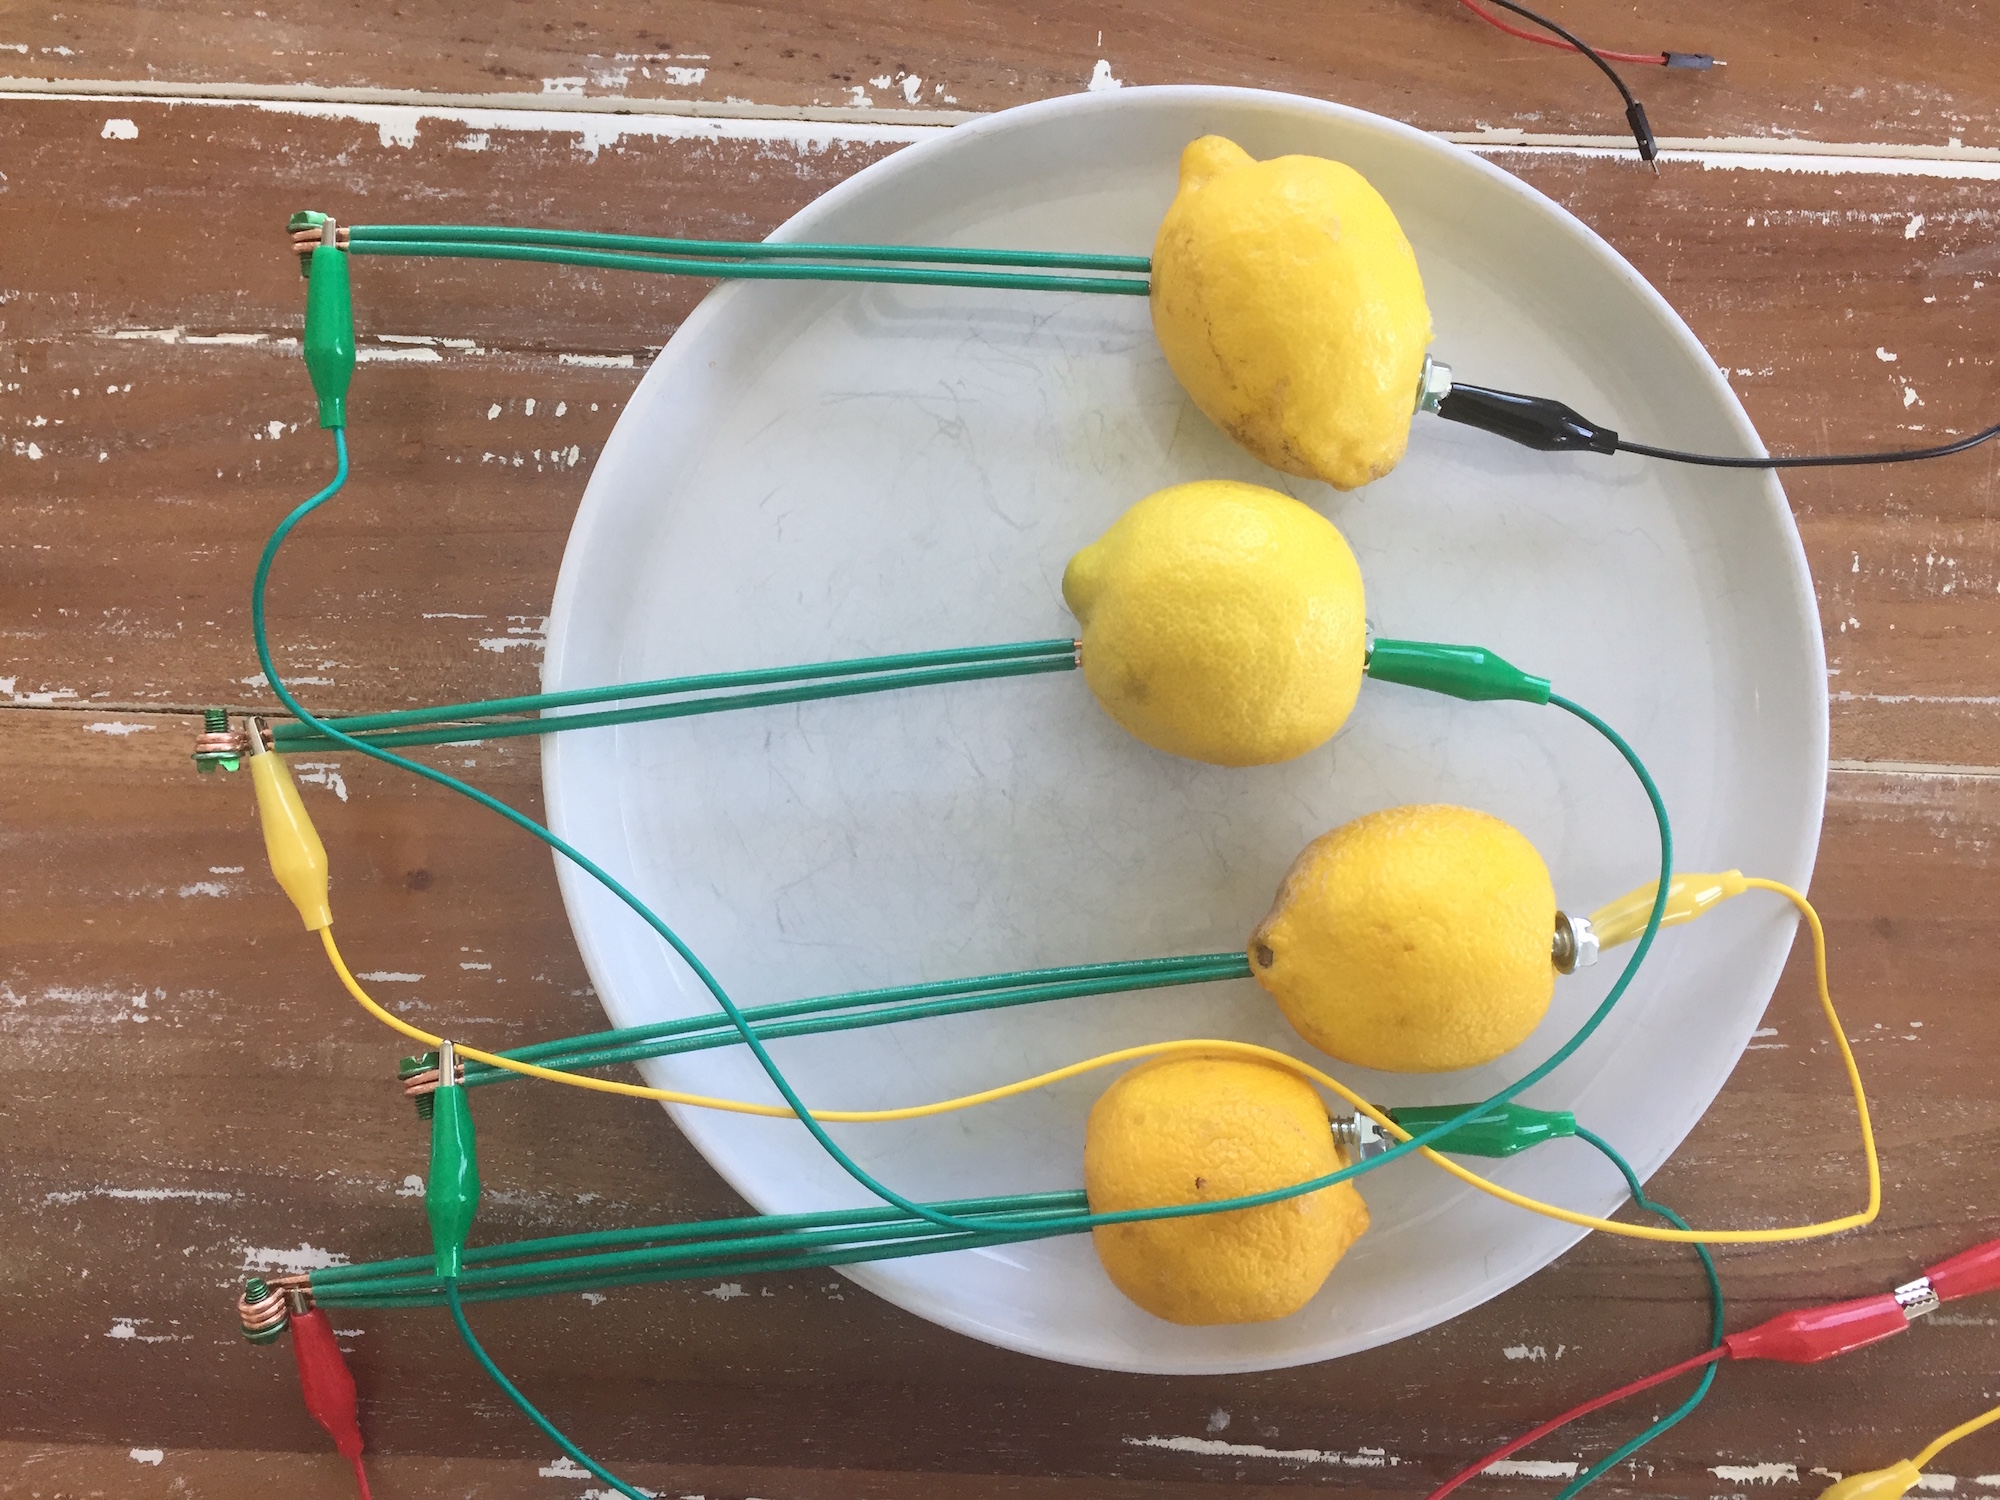
\includegraphics[scale=0.14]{4lemonbattery.jpg}
}
\medskip
\caption{This four-lemon battery was constructed using large zinc-coated sheet metal screws and copper grounding stakes (the plastic coating does not extend all the way down the stake). Together, the lemons made about 4 volts (open circuit / no load) and was just barely able to light up an LED.}
\end{center}
\end{figure}


\subsection*{Charge}

Electric charge is a basic property of electrons and protons. Electrons are negatively charged and protons are positively charged. Things that are negatively charged and things that are positively charged pull on (attract) each other. Things that have the same charge push each other away (they repel each other). This behavior is called the \emph{Law of Charges}. Things that have equal numbers of electrons and protons are neutral. Things that have more electrons than protons are negatively charged, while things with \emph{fewer} electrons than protons are positively charged. 

%Lightning strikes result when a huge charge up in a cloud overcomes the natural resistance of the air and the electricity reaches towards the ground, since the ground is charged positively

%Exact values of charge strength in each of the regions varies, but a charge of $+40$ coulombs has been suggested as a typical value for the P-region (near top of cloud) and $-40$ coulombs for the N-region (near bottom of cloud) and $+10$ coulombs for the p-region (small p - near lower portion of rain area). One coulomb is the amount of charge which is moved past a given cross-section of wire when a current of 1 ampere flows for 1 second.

\subsection*{Voltage}

Voltage is a force that makes electricity move through a wire. It is measured in volts. Voltage is also called \emph{electric tension} or \emph{electromotive force} (EMF). It was named after Alessandro Volta.

Though it's not the most helpful definition, the best definition of voltage is \emph{the difference in electric potential between two points}. Voltage is always measured between two points, for example between the positive and negative ends of a battery, or between a wire and ground. 

The most common analogy for electricity is water in pipes. If we think of water in pipes, voltage is the \emph{water pressure} pushing on the water to get it to move through the pipes. Voltage is proportional, meaning that 3 Volts pushes twice as hard on electrons (to get them to move) as 1.5 Volts pushes.

Static shocks, like the kind you get on metal surfaces in the winter when wearing a wool sweater, can be up to 30,000 volts -- but it's not dangerous to you because the amount of electrical charge is so small. The voltage has a very high \emph{potential}, but cannot do much work.

\bigskip

\stbox{6.0in}{\emph{Experiment:} Push 9V battery terminals into your arm. Then lick the 9V battery terminals. Why did you feel the electricity on your tongue and not your arm? 
}


\subsection*{Current}

An electric current is a flow of electric charge. The SI unit of electric current is the \emph{ampere} (A), almost always shortened to ``amp''. This is equal to one coulomb of charge in one second. A coulomb is an exact count of electron charges (6,241,509,629,152,650,000 elementary charges -- that's over six quintillion electrons!). Electrons are very small, and contain only a very, very tiny amount of charge. An amp of current can be a lot or a little, depending on how much voltage is pushing the current. 5 amps at 2,000 volts would kill you. 1 amp at 5 volts can't even shock you. Smaller currents than one amp are usually measured in \emph{milliamps}, or one-thousandths of an amp. So 500 milliamps is half an amp. 100 milliamps is a tenth of an amp. Milliamps are usually abbreviated ``mA".

\bigskip

\stbox{6.0in}{\begin{Large}

{\color{red}Electricity can be dangerous. Never work with electricity unless an adult has shown you how to be safe, and told you the work you are doing is safe.}

\end{Large}

\begin{center}
{\color{red} A little saying to help remember how electricity can be dangerous is:

\bigskip

\textbf{``volts jolt; mils [milliamps] kill."}}
\end{center}

That is, even high voltages like static electricity shocks are not necessarily dangerous, but even low currents can be deadly.
}



\subsection*{Resistance}

Resistance is how much a material or component prevents the flow of electricity. Substances with very, very high resistances are \emph{insulators} -- they prevent the flow entirely under most conditions. Substances that pass electricity at least some are called \emph{conductors}. Copper, silver, and gold are excellent conductors. Aluminum, zinc, and iron are good conductors too, but not all metals are good conductors. Titanium is a poor conductor, but is not an insulator. 

Many resistors are made with some amount of carbon inside them -- carbon conducts electricity but not very well. The more carbon between the wires, the higher the resistance. Modern resistors don't necessarily use carbon, but it is still used. While a resistive material does pass electricity, it also slows down the flow, and prevents some electricity from passing. This electricity that gets ``used up'' by the resistor is turned into heat. 

\stbox{6.0in}{\emph{Experiment:} A salt-water resistor. Attach wires to an LED (without the resistor this time, which is normally a bad idea). Hook the positive end to a 3 to 5 volt supply, leaving the negative terminal open. Drop one wire from the negative terminal of the LED into a glass jar half-full of (distilled, if you have it) water. Tape the wire to the lip of the jar, and make sure the wire is submerged. Put the wire from the negative terminal in the jar, under water, but keep the wires pretty far apart. Does the LED come on? Would you expect it to? Now add some salt to the water. What happened? (May need to add more salt). }

\subsection*{Ohm's Law}

Electricity and electronics can be understood using many equations, but we'll only look at one of them. \emph{Ohm's Law} says that the voltage, current, and resistance in a circuit are all related, in a way that can be calculated because the values are related in a knowable proportion. Ohm's Law states that the current through a conductor (wire) between two points is directly proportional to the voltage across the two points.

The law was named after a German scientist, Georg Ohm, who wrote an early book about electricity in  1827. He described measurements of voltage and current through simple electrical circuits containing various lengths of wire.

If we abbreviate ``voltage" to V, ``resistance" to R, and use I for ``current" (the scientist who first understood current pretty well was French, and he referred to current as \emph{intensit{\'e} de courant}, meaning ``current intensity", so we use ``I'' for current). 

\begin{equation}
V = I \times R
\end{equation}


That is, voltage is equal to however much current is flowing, times how much total resistance is in the circuit. Because the individual components are proportional, the law can be written other ways:

\begin{equation}
I =  \frac{V}{R}
\end{equation}

One very practical application of Ohm's law is that it allows an engineer to limit how much current can flow in a circuit by adding a certain level of resistance. Often it would be safer to keep a lot of current from flowing, so even a little extra resistance can make the circuit (and the components in the circuit) safer and more durable. Resistors consume some energy, and turn electricity into heat.



